
\documentclass{beamer}
\mode<presentation>
\usepackage{amsmath}
\usepackage{amssymb}
%\usepackage{advdate}
\usepackage{graphicx}
\graphicspath{{../figs/}}
\usepackage{adjustbox}
\usepackage{subcaption}
\usepackage{enumitem}
\usepackage{multicol}
\usepackage{mathtools}
\usepackage{listings}
\usepackage{url}
\def\UrlBreaks{\do\/\do-}
\usetheme{Boadilla}
\usecolortheme{lily}
\setbeamertemplate{footline}
{
  \leavevmode%
  \hbox{%
  \begin{beamercolorbox}[wd=\paperwidth,ht=2.25ex,dp=1ex,right]{author in head/foot}%
    \insertframenumber{} / \inserttotalframenumber\hspace*{2ex} 
  \end{beamercolorbox}}%
  \vskip0pt%
}
\setbeamertemplate{navigation symbols}{}
\let\solution\relax
\usepackage{gvv}
\lstset{
%language=C,
frame=single, 
breaklines=true,
columns=fullflexible
}

\numberwithin{equation}{section}
\title{5.2.68}
\author{AI25BTECH11001 - ABHISEK MOHAPATRA}
% \maketitle
% \newpage
% \bigskip
\begin{document}
{\let\newpage\relax\maketitle}
\renewcommand{\thefigure}{\theenumi}
\renewcommand{\thetable}{\theenumi}



	 	\textbf{Question}:
		Solve $2x + 3y = 11$ and $2x + 4y = -24$ and hence find the value of $m$ fror which $y = mx + 3$.

		\textbf{Solution:}
		Given:
		\begin{align}
				2x +3y = 11
		\end{align}And,
		\begin{align}
				2x + 4y = -24
		\end{align}So,
		\begin{align}
				\myvec{ 2 &3\\2&4}\vec{X} = \myvec{11 \\ -24}
		\end{align}
		Augumented Matrix:
		\begin{align}
				\augvec{2}{1}{2 & 3 & 11\\2&4&-24}
		\end{align}
		\begin{align}
				\xrightarrow[]{R_2\rightarrow R_2-R_1}\augvec{2}{1}{2 & 3 & 11\\0&1&-35}
		\end{align}
		\begin{align}
				\xrightarrow[]{R_1\rightarrow R_1-3R_2}\augvec{2}{1}{2 & 0 & 116\\0&1&-35}
		\end{align}
		\begin{align}
				\Rightarrow \augvec{2}{1}{1 & 0 & 58\\0&1&-35}
		\end{align}
		So, 
		\begin{align}
		\vec{X} = \myvec{x\\y} = \myvec{58\\-35}
		\end{align}
		Given,
		\begin{align}
		y = mx+3
		\end{align}
		\begin{align}
		\Rightarrow m = \frac{y-3}{x} = - \frac{19}{29}
		\end{align}
		So, m = $-\frac{19}{29}$


Graph:
\begin{figure}[h!]
	\centering
	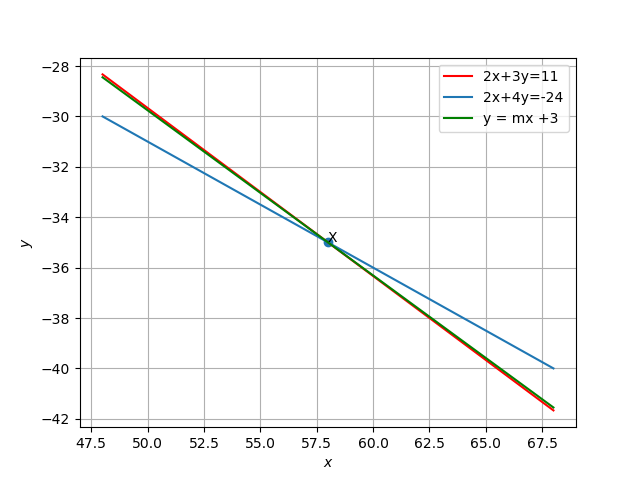
\includegraphics[width=0.7\linewidth]{img.png}
\end{figure}	
\end{document}


